\documentclass{article}

\usepackage[utf8]{inputenc}
\usepackage{amsmath}
\usepackage{amsfonts}
\usepackage{amssymb}
\usepackage{algorithm}
\usepackage{algorithmic}
\usepackage{german}
\usepackage{color}
\usepackage{bbm}
\usepackage{makeidx}
\usepackage{graphicx}

\title{Small summery}
\author{Boris Prochnau}
\begin{document}
\maketitle
\tableofcontents
\section{First meeting (14.04): Model of interest}
These are some main points of the model we are using for the simulation. They are the product of the first meeting with Loren Coquille and Martina Baar.
\begin{itemize}
	\item We have N traints and ($X_{i=1,...,N}$) are the amount of members of the traits. 
	\item We use a constant mutation rate that does not depend on the traits $\mu$.
	\item but the other rates are depending on traits and change with time (by as the amount of traitmembers rises)
		\begin{itemize}
			\item $b_i$, [intrinsic birth-rate]
			\item $d_i$, [intrinsic death-rate]
			\item $\left(\sum_{j=1}^N \frac{c_{\cdot,j}}{K}x_j\right)_i$, [competition death]
			\item $\mu\left(\frac{b_{i-1} + b_{i+1}}{2}\right)$, [extrinsic birth-rate]
		\end{itemize}
	\item We use 3 groups of PPP's where every group represents an event. 
		
		\begin{itemize}
			\item $N_t^{b_i}$
			\item $N_t^{d_i}$
			\item $N_t^{\bar{c}_i}$
		\end{itemize}
	where $\bar{c} = \left(\sum_{j=1}^N \frac{c_{\cdot,j}}{K}x_j\right)_i$. Therefore we get 3N processes running that compete about the first one occurring with each one triggering an death/birth for an trait.
	\item With respect to the fact that the distribution of the $N_t$ changes with the size of the population we can think of an reset of the parameters of $N_t$ due to the fact that the increments are exponentially distributed and therefore are memoryless (markov property)
	\item The use of coloring one trait was (only $\to$ ask later) to explain the superposition of the PPP associated with the simulation to extract the occured event from the PPP's \\
	\[\to N_t^{total_{i}} = N_t^{b_i + d_i + \bar{c}_i} = N_t^{b_i} + N_t^{d_i} + N_t^{\bar{c}_i}\]
Therefore we would decide:
\begin{equation}
	X_i^{total} = 
	\begin{cases}
		\textrm{coloring d} & \textrm{with prob. p}\\
		\textrm{coloring b} & \textrm{with prob. q} \\
		\textrm{coloring }\bar{c} & \textrm{with prob. 1-p-q}  
	\end{cases}
\end{equation}
with:
\begin{align*}
	p = \frac{d_i}{d_i + b_i + \bar{c}_i} && q = \frac{b_i}{d_i + b_i + \bar{c}_i} && 1-p-q = \frac{\bar{c}_i}{d_i + b_i + \bar{c}_i}
\end{align*}
\end{itemize}

\section{Second meeting (22.04): Pseudocode}
First thing to mention is that the Pseudocode snippets are marked as "`Algorithm"', but in fact they are just functions and I don’t know yet how to change the name in this particular LaTeX environment. Also I use a "`="' instead of "`$\leftarrow$"' because I think it provides better readability.\\
The following Pseudocode will contain many function-calls. Every function can be identified as a verb, and objects or local variables are nouns. There will also be one Boolean "`isBorn"' which is an adjective.\\
Generally the functions have no return values because in this situation we tell functions to do something (not ask). Means we pass a task to them. There will be no requests for return values.\\
One other thing to mention is that the function names can get long, but they will (or should) always say what the function does. Not more or less.\\
The function-body should always follow a rule called "`pretty much what you expected"'. Some functions do violent this rule slightly. They are usually more than 6 lines and will be changed later.\\
First we start with the main Step of the Algorithm and continue with further explaining of the used functions. When a new function appear, it will be explained directly below it. Also we seperate this section in 3 parts, each one is dedicated to one of the functions used in this following EvolutionStep():
\begin{algorithm}[H]
	\caption{EvolutionStep()}
	\begin{algorithmic}[1]
		\REQUIRE -
		\ENSURE{A full evolution Step happened}
		\STATE calculateEventRates();
		\STATE sampleEventTime();
		\STATE changeATrait();
	\end{algorithmic}
\end{algorithm}
This function does a full evolution step. First thing to do is to calculate the Event rates with "`calculateEventRates"', than we sample an exponential time with our current rate parameters with "`sampleEventTime"' and finish the Step with changing a Trait with "`changeATrait"'. \\
Most functions-calls should not need to be explained, that’s why I leave this explanations out in following comments.\\
This function will be improved later with not calculating the Rates in every new step, rather than updating them with the previous changes. \\
	
\subsection{Calculating total-event rates}
We will encounter 2 classes called "`Trait"' and "`Events"'. They are so called Data Classes and usually mainly store data.\\
They are visible at all time and can be used like global variables. \\
In this first part of calculating total-event rates we only need to introduce the "`Trait"' class which will be used as an array of traits "`Trait[$i\le n$]"' with n beeing the maximum number of traits. An Trait Object has attributes that can be accessed through a dot operator like "`Trait[i].Members"' what would be "`the Members of Trait i"'.\\
This is a listing of all attributes in one Trait Object:\\
\textcolor[rgb]{0,0,0.55}{\textbf{class Trait}
\begin{itemize}
	\item BirthRate
	\item TotalBirthRate
	\item DeathRate
	\item TotalDeathRate
	\item TotalTraitRate
	\item TotalEventRate - [static]
	\item CompDeathRate[i][j] - [static]
\end{itemize}
}

Here is much work with Superposition of the PPP included. We summarize the sum of birth-rates from members within a trait to the "`TotalBirthRate"' (mutation included), same for "`TotalDeathRate"' (competition included). \\
The "`TotalTraitRate"' is the summed  "'TotalBirthRate"' and "`TotalDeathRate"' and means the total rate of events for a specific trait. \\
"`TotalEventRate"' and "`CompDeathRate"' are static, this means that they are the same for all initialized Trait objects. They (all items from the array) access the same variable for this. "`TotalEventRate"' is the same as usual and "`CompDeathRate"' is the competition-matrix with according rates.\\	
\begin{algorithm}[H]
	\caption{calculateEventRates()}
	\begin{algorithmic}[1]
		\REQUIRE -
		\ENSURE{All (total)Rates will be set}
		\FOR{i=0 \TO n-1}
			\STATE calculateTotalDeathRateOf(i)
		\ENDFOR
		\STATE calculateTotalBirthRates(0);
		\STATE calculateTotalEventRate();
	\end{algorithmic}
\end{algorithm}
In the next function we will manipulate attributes of the Trait Objects. The mutation will be accessed without and Traitindex: "`Trait.Mutation"' because it is static and therefore the same for all Objects.
\begin{algorithm}[H]
	\caption{calculateTotalBirthRates(StartIndex: i)}
	\begin{algorithmic}[1]
		\REQUIRE int i
		\ENSURE{Total birthrate of Trait "`i"' will be set (recursively)}
		\STATE Trait[i].TotalBirthRate = (Trait[i].Members)$\cdot$(Trait[i].BirthRate)
		\IF{$i < n-1$}
			\STATE calculateTotalBirthRates(i+1)
			\STATE Trait[i].TotalBirthRate += $\frac{Trait.Mutation}{2}\cdot Trait[i+1].TotalBirthRate $
		\ENDIF
		\IF{$i > 0$}
			\STATE Trait[i].TotalBirthRate += $\frac{Trait.Mutation}{2}\cdot Trait[i-1].TotalBirthRate $
		\ENDIF
	\end{algorithmic}
\end{algorithm}
In Algorithm 3 in line 3 is used recursion, because this improves the calculation speed a lot, although it slightly makes code less intuitive.

\begin{algorithm}[H][H]
	\caption{calculateTotalDeathRateOf(TraitIndex: i)}
	\begin{algorithmic}[1]
		\REQUIRE int i
		\ENSURE{Total deathrate of Trait "`i"' will be set}
		\STATE Trait[i].TotalDeathRate = 0;
		\STATE addTotalIntrinsicDeathRateOf(i);
		\STATE addTotalCompetitionDeathRateOf(i);
	\end{algorithmic}
\end{algorithm}

\begin{algorithm}[H]
	\caption{addTotalIntrinsicDeathRateOf(TraitIndex: i)}
	\begin{algorithmic}[1]
		\STATE Trait[i].TotalDeathRate = (Trait[i].DeathRate) $\cdot$ (Trait[i].Members)
	\end{algorithmic}
\end{algorithm}
\begin{algorithm}[H]
	\caption{addTotalCompetitionDeathRateOf(TraitIndex: i)}
	\begin{algorithmic}[1]
		\FOR{j=0 \TO n-1}
			\STATE Trait[i].TotalDeathRate += (Trait.CompDeathRate[i,j])$\cdot$(Trait[j].Members);
		\ENDFOR
	\end{algorithmic}
\end{algorithm}

\begin{algorithm}[H]
	\caption{calculateTotalEventRate()}
	\begin{algorithmic}[1]
		\REQUIRE -
		\ENSURE{Current Totaleventrate is set}
		\FOR{i=0 \TO n-1}
			\STATE Trait[i].TotalTraitRate = Trait[i].TotalBirthRate \\ 
			\noindent\hspace*{36mm}+ Trait[i].TotalDeathRate;
			\STATE Trait.TotalEventRate += Trait[i].TotalTraitRate;
		\ENDFOR
	\end{algorithmic}
\end{algorithm}

\subsection{Sampling the next event-time}
Here will appear a, not yet mentioned, object that will not be explained further, called Dice. The Dice Object will provide a uniform or exponential random Variable.\\
\begin{algorithm}[H]
	\caption{sampleEventTime()}
	\begin{algorithmic}[1]
		\REQUIRE -
		\ENSURE{First ringing Eventclock has been sampled}
		\STATE double Parameter = Trait.TotalEventRate;
		\STATE double newEvent = this.Dice.RollExpDice(Parameter);
		\STATE Events.EventTimes.push(newEvent);
	\end{algorithmic}
\end{algorithm}
Here we use Dice.RollExpDice($\lambda$) to get $X\sim exp(\lambda)$. The same is possible for  Dice.RollUnifDice($\lambda$) to get $X\sim Unif[0,\lambda]$.\\

\subsection{Changing a trait}
Here we will work with the actual Events taking place. For this purpose i introduce the Events class like before the Trait class:\\
\textcolor[rgb]{0,0,0.55}{\textbf{class Events}
\begin{itemize}
	\item Dice
	\item EventTimes[i]
	\item ChosenTrait[i]
	\item isBirth[]
\end{itemize}
}
The EventTime, ChosenTrait and isBirth are so called vectors. They are dynamic containers and we need to push an item into them to append it to the last entry.
\begin{algorithm}[H]
	\caption{changeATrait()}
	\begin{algorithmic}[1]
		\REQUIRE -
		\ENSURE{make a change to the Population with current Parameters}
		\STATE choseTraitToChange();
		\STATE choseEventType();
		\STATE executeEventTypeOnTrait();
	\end{algorithmic}
\end{algorithm}

\begin{algorithm}[H]
	\caption{choseTraitToChange()}
	\begin{algorithmic}[1]
		\REQUIRE -
		\ENSURE{Trait is chosen for changing}
		\STATE double Parameter = Trait.TotalEventRate;
		\STATE double HittenTrait = Dice.rollUnif(Parameter);
		\FOR{i = 1 \TO n-1}
			\IF{HittenTrait $\le$ Trait[i].TotalEvent}
				\STATE this.ChosenTrait.push(i);
				\STATE break;
			\ENDIF
			\STATE HittenTrait -= Trait[i].TotalEvent;
		\ENDFOR
	\end{algorithmic}
\end{algorithm}

\begin{algorithm}[H]
	\caption{choseEventType()}
	\begin{algorithmic}[1]
		\REQUIRE -
		\ENSURE{Decision for Birth or Death is made}
		\STATE int i = Events.ChosenTrait.lastentry();
		\STATE double EventType = Dice.rollUnif(Trait[i].TotalTraitRate);
		\IF{EventType $\le$ Trait[i].TotalBirthRate}
			\STATE Events.isBirth.push(true);
		\ELSE
			\STATE Events.isBirth.push(false);
		\ENDIF
	\end{algorithmic}
\end{algorithm}

\begin{algorithm}[H]
	\caption{executeEventTypeOnTrait()}
	\begin{algorithmic}[1]
		\REQUIRE -
		\ENSURE{Chosen event will occur on chosen trait}
		\IF{isBirth}
			\STATE Trait[ChosenTrait.lastentry()] += 1;
		\ELSE
			\IF{ChosenTrait.Members $>$ 0}
			\STATE Trait[ChosenTrait.lastentry()] -= 1;
			\ENDIF
		\ENDIF
	\end{algorithmic}
\end{algorithm}
\listofalgorithms

\newpage
\section{Thrid and Fourth meeting (Di 20.05 and 13.05): Graphical plans - afterwards}
Zunächst habe nicht meine bisherigen Fortschritte präsentiert. Dazu gehörte ...\\
Außerdem haben wir die graphischen Ansprüche an das Programm besprochen.
Dabei wurden folgende Ergebnisse erzielt:
\begin{itemize}
\item Man sollte eine gute Möglichkeit haben die Parameter im Programm einsehen zu können und auch eine gute Möglichkeit Daten zu laden.
\item Was besonders wertvoll ist, wäre eine Möglichkeit neue Instanzen zu generieren. Dabei hat sich jedoch das Problem gestellt dass es keine einfache Konsole mit simplem einseitigen Output und Input gibt, da man während einer Instanzgenerierung auch weiterhin mit dem Hauptfenster interagieren könnte. Das Problem wurde etwas umständlich über eine kontrollierte Deaktivierung der anderen Interfaceelemente gelöst.
\end{itemize}
Zur Darstellung des Graphen wurde folgendes gesagt:
\begin{itemize}
\item Es ist keine "{}Filmfunktion"{} gewünscht. Stattdessen sollte man einen Plot generieren und in diesen hereinzoomen und mit der Maus ziehen können.
\item Außerdem ist eine Legende gewünscht die eine Übersicht über alle Graphen bietet. 
\item Um die Graphen später vergleichen zu können sollte es eine Möglichkeit geben den Graph zu speichern.
\end{itemize}

\newpage
\section{Fifth meeting (Fr 30.05): Improvements - afterwards}
An diesem Tag habe bloß einige Änderungen vorgestellt und sichergestellt dass alle Funktionen ordnungsgemäß laufen:
\subsection{Graphische Änderungen}
Das waren hoffentlich alle optisch merklichen Änderungen:
\begin{itemize}
\item Ich habe eine Checkbox hinzugefügt die eine Option für sinnvollen Abbruch bietet. Diese Funktion prüft ob sich beide Populationen in einer $/epsilon$ Umgebung um den erwarteten Zustand befindet und stoppt anschließend die Iterationen. Zu Gunsten der Übersicht werden noch mal 1/3 der Anzahl bisher gemachten Iterationen angefügt.\\
Zu diesem Zeitpunkt ist $\epsilon = \frac{5}{\sqrt{K}}$.
\item Es wurde ein Anzeigefehler behoben der für Geburts- und Todesraten immer nur die Populationsgrößen der Eigenschaften angezeigt hat.
\item Auf dem Plotfenster habe ich ein Label mit den gemachten Iterationen hinzugefügt. Weiterhin findet sich dort jetzt auch ein Feld wo man einen Dateinamen eingeben kann der einem gespeichterten Bild dienen soll welches man mit dem neuen "{}save Image"{} Button erstellen kann. Das Bild wird zur Zeit als .png und .pdf gespeichert.
\item Die x-Achsenbeschriftung lautet nun nicht mehr Millisekunden sondern "{}Time"{}. Grund dafür ist dass ich nicht sicher bin welche Zeit unsere exponentielle Uhr ausgibt. Jedoch habe ich sie der Übersicht halber nicht mehr durch 1000 geteilt, da bei den gewünschten Instanzen ausreichend große Zeiten angenommen werden.
\item Zuletzt wurde noch bei der Legende der für die k-te Erwartete Eigenschaft "{}k. Expected"{} zusätzlich der konvergierte Wert angezeigt "{}k. Exp: 1.048"{}.
\end{itemize}

\subsection{Interne Änderungen}
\begin{itemize}
\item Ich habe mehrere Arten der Datenspeicherung ausprobiert. Zunächst habe ich die Daten alle nacheinander in eine "{}Storage"{} Datei geschrieben um schließlich einzeln die Daten mit "{}addData"{} zum Graphen hinzuzufügen. Das schien mir jedoch an der "{}addData"{} Stelle und am Datastream zu aufwendig.  
Danach bin ich auf eine alternative mit "{}Jumped Steps"{} umgestiegen. Die Jumped Steps basieren darauf das maximal 10.000.000 Punkte gespeichert werden und auch wenn viel mehr Iterationen gemacht werden, so werden nur Äquidistante 10 mio Stützstellen geplottet. Der Gedanke dahinter war die nicht Unterscheidbarkeit des Graphen für das menschliche Auge.
\item Ich habe eine "{}GraphClass"{} hinzugefügt die alle Daten für das "{}PlotWindow"{} vorbereitet, so dass das Fenster nur noch darauf zugreifen muss. Damit habe ich eine Brücke zwischen den Fenstern und dem Plot geschlagen.
\item Eine der wichtigsten Änderungen ist das Hinzufügen des QThreads. Dieser gewährleistet dass der Plot die Fenster nicht einfrieren lässt. Die Berechnung kann für mehr als 1mio Punkte bereits merkliche Zeit (>3s) beanspruchen.
\item ...to do...
\end{itemize}

\subsection{bekannte Bugs}
Es gibt hier noch einen Bug der mit der Beschriftung der x-Achse zu tun hat. Ich weiß noch nicht wie man ihn reproduziert, aber er könnte die Achse um einen großen Faktor zu groß skalieren. Der Plot weißt jedoch das geplante Verhalten auf und dieser Bug tritt nur bei \"replots\", also dann auf wenn ein neuer Plot den alten überschreibt.

\newpage
\section{Sixth meeting (03.06): Introducing TSS}
Einführung in TSS
\begin{itemize}
\item Das erste war das Einfügen einer Tabelle oder Grafik die einen guten Überblick über die Fitness der Population bietet. Diese gibt Aufschluss darüber ob TSS ordnungsgemäßes Verhalten zeigen wird. Allgemein ist es aber auch gut zu sehen welche Population wie stark auf eine andere wirkt, daher vielleicht schon ohne TSS sinnvoll.\\
Um eine bessere Übersicht von ungewünschtem Verhalten zu zeigen werden Coexistenzen rot markiert. Später wird noch eine weitere grünliche Färbung angezeigt die eine Verdrängungswahrscheinlichkeit darstellt.
Dieses Feature wird in beiden Programmen vorhanden sein.\\
Die verwendete Formel zur Berechnung der Fitness war \[ f_{x,y} = b_x - d_x - c_{x,y}\cdot \bar{n}_x\]
mit:
\[ \bar{n}_x = \frac{b_x - d_x}{c_{x,x}}\]
Demnach wird auf der Diagonale stets eine Null erwartet. Bei dieser Rechnung tritt jedoch eine Subtraktion auf die Auslöschung verursacht. Zu diesem Zweck habe ich die dargestellte Zahl auf 14 stellen runden lassen.
\item Ein besseres Verständnis von TSS wäre nützlich. Dazu wurde mir aus [2] S.1135 empfohlen. Leider habe ich es bisher noch nicht geschafft es durchzuarbeiten. Es wird auf den nächsten Wochenplan kommen.
\item Außerdem wurde die Skalierung der Mutationswahrscheinlichkeit mit K angepasst so dass TSS realistisch laufen kann. Dabei wurde der Faktor $\frac{1}{K^{1.5}}$ gewählt weil es den notwendigen Schranken die in [2] S.1135 beschrieben werden genügt. Ein weiterer Punkt den man optimieren kann wäre es eine Option zur Eingabe eines eigenen Exponenten für K wäre eine mögliche Erweiterung.
\item In diesem Zustand ist es bereits Möglich einen TSS plot zu erzeugen. Jedoch wird die Zeit im Equilibrium tatsächlich berechnet was viel unnötige Rechenarbeit impliziert. Später solle eine lineare Interpolation bis zur ersten Mutation gemacht werden sobald das Equilibrium erreicht wird.  
\subsection{Bekannte Bugs}
Es ist ein Bug bisher übrig. Bisher kenne ich noch nicht den Ursprung, aber er äußert sich (meistens) durch einen Programmabsturz nachdem ich eine kleinere Instanz lade und anschließend TSS1 bzw eine größere Instanz lade. Der Plot wurde dabei noch nicht ausgeführt.
\end{itemize}
  
\newpage
\section{Seventh meeting (10.06): Bug fixing and interpolation of Equilibrium}
\subsection{Was ist geplant?}
Geplant ist:
\begin{itemize}
	\item Beheben eines Fehlers beim Laden der Instanzen. Dieser wurde im letzten Kapitel beschrieben.
	\item Eine lineare Interpolation der Population im Equilibrium. Die Funktion dazu wurde bereits geschrieben.
	\item Korrekte Ausarbeitung eines geeigneten Abbruchkriteriums für TSS Prozesse.
	\item Punkte an denen eine Mutation stattgefunden hat sollen idealerweise hervorgehoben werden. Z.B. durch kreuze oder ähnliches.
	\item Am Besten wäre noch eine Skalierung der Zeitachse während des Equilibriums. 
	\item Die Fitnessmatrix sollte bisher eine Bandmatrix sein weil es nur Mutationen zum Nachbarn gibt.
\end{itemize}

\subsection{Was habe ich gemacht?}
Konkret:
\begin{itemize}
	\item Bisher habe ich eine Neudefinition der "{}isNear()"{} Funktion gemacht. Diese gibt es nun als "{}isNearDimorph()"{}, "{}isNearMonomorph()"{} und "{}isNearTSS()"{}. Diese tun was man vom Namen her erwartet, wobei "{}isNearTSS()"{} prüft die Nähe zum Equilibrium bzw. es prüft ob die Population bereits auf das Equilibrium getroffen ist (mit Rücksicht auf Auslöschung bis zu einer Genauigkeit von $10^{-10}$) und ob die Population zur Zeit die einzig aktive ist. 
	\item Weiterhin existiert eine neue Version der "{}iterateGraphPoint()"{} Methode. Sie heißt "{}iterateMutationPoint()"{} und soll den Zeitpunkt der nächsten Mutation der Nachbarn berechnen. Anschließend soll dieser Zeitpunkt in der Zeitlinie gespeichert werden und dort eine Mutation auf der Population ausgeführt werden.
	\item Diese "{}iterateMutationPoint()"{} Funktion soll anschließend von einer neuen Funktion "{}makeTSSIterations()"{} nur dann ausgeführt werden, wenn die neue "{}isNearTSS()"{} eine Bestätigung liefert.
	All diese Änderungen wurden in der GraphClass gemacht und werden in "{}generateEvolution()"{} verwendet.
	\item Ein wichtiger Zusatz für die Berechnung der Geburtenrate wurde getroffen. Dabei wurde jetzt nicht mehr zu beginn $b(i)\cdot N(i) + MutationFromNeighbors$ gerechnet, sondern $b(i)\cdot N(i) \cdot (1-\mu) + MutationFromNeighbors$. Das ist bisher nicht aufgefallen weil $\mu$ für gewöhnliche dimorphe Prozesse immer Null war.
	\item Eine sehr wichtige Änderung sollte die Berechnung des monomorphen stabilen Zustands gelten. Wenn eine positive Mutationswahrscheinlichkeit vorliegt, so sinkt die Arteigene Geburtenrate um die Mutationswahrscheinlichkeit. Somit berechnet sich das Equilibrium im TSS durch \[\frac{b(x)\cdot (1-\mu) - d(x)}{c_{x,x}}\]
	\item NearTSS wurden die Grenzen geändert, so dass es jetzt eine Umgebung von 1/K um das Equilibrium gibt statt dem genauen Treffer. Das ist notwendig, weil es sein kann dass unser Equilibrium kein Vielfaches von 1/K ist, gewährleistet aber trotzdem die gröst mögliche Nähe zum Equilibrium.
	\item Es hat sich ein Bug ergeben der die Zeit falsch (bzw immer mit der ersten Rate) berechnet hat. Das wurde durch ein veraltetes "{}static"{} beim Ziehen der Würfelergebnisse verursacht.
	\item Ein weiteres Problem wurde behoben nach dem zufolge es noch keine ordentlich Anzeige für ein TSS gab, nachdem ein Trait zum ersten mal ausgestorben ist. Die Ursache lag in der "{}isNearTSS()"{} Funktion, daher wurde diese Überarbeitet.
	\item Es gab ein Problem weshalb der angezeigte stabile Zustand nicht bis zum Mutationspunkt durchgezogen wurde, sondern bereits sichtbar davor stoppte. Die Ursache war dass nur die Zeit bis zur nächsten Mutation als neuer Zeitpunkt gespeichert wurde, nicht aber die iterierte Zeit.
	\item Ich habe einen Bug behoben der das Programm manchmal zum Absturz brachte. Dabei handelte es sich wahrscheinlich um einen Speicherfehler, die genaue Ursache kenne ich nicht, aber ich konnte den Fehler beheben indem ich die Fitness Matrix "{}gecleart()"{} habe bevor sie erneut "{}resize()"{} aufruft.
\end{itemize}
todo
\begin{itemize}
 \item Es sollten direkte getter und setter auf die Trait und Event Members ausgeführt werden satt sie temporär zu speichern wie in "{}generateEvolution()"{}. 
\end{itemize}
\subsection{Bekannte Bugs}
\begin{itemize}
	 \item Der letzte Punkt des Graphen wurde nicht gespeichert. Außerdem sollte der Graph auch wenn nichts mehr für ihn passiert, trotzdem bis zum ende fortgesetzt werden. Dazu sollte der letzte Zeitpunkt nocheinmal mit dem Endzustand abgespeichert werden. 
	 \item Exp in der Legende sollte gesondert geändert werden.
	 \item Problem mit K-member K-expected und Darstellung beider.
\end{itemize}

\newpage
\section{Zweites Bachelorseminar - Simulation der normalisierten BPDL und TSS Prozesse}
Der Inhalt dieses Vortrags soll zeigen was ich bisher gemacht habe und welches Ziel ich damit verfolge. Leider erlaubt die Zeit keinen detaillierten Einblick\\
Den größten Teil der Zeit seit dem letzten Seminar habe ich mit programmieren Verbracht. Daher wird ein größerer Teil am Ende dem Ergebnis dieser Arbeit gewidmet.\\
Zu Beginn möchte ich jedoch nochmal kurz eine etwas andere Darstellung des zuletzt vorgestellten Models mit einigen Einschränkungen präsentieren.
	\subsection{Ziel}
		Das Ziel meiner Bachelorarbeit ist es ein Programm zu entwickeln welches eine Simulation eines normalisierten BPDL und TSS Prozesses durchführen kann. Dies soll dem besseren Verständnis über BPDL und TSS Prozessen dienen (und kann zu statischen Nachweisen verwendet werden). Gerade deswegen ist es wichtig sicherstellen zu können dass sich keine Fehler in die Implementation einschleicht. Dazu jedoch mehr im Kapitel "{}Korrektheit der Implementation"{}.
	\subsection{Model}
		Zunächst möchte ich das in der Simulation verwendete Model vorstellen.\\
		\begin{itemize}
			\item Dieses Modell soll eine Population beschreiben in der jedes Individuum ein Merkmal $ x \in X \subset \mathbf{R}^n $ hat. Wobei die Simulation $ X $ ein endlichen diskreten Merkmalsraum verwendet der hier der Einfachheit halber als Indexmenge $ X = \{1,\dots, n\} $ repräsentativ für eine Durchzählung der Merkmale steht.
			\item Jedes Individuum kann sich entweder asexuell fortpflanzen oder sterben
			\item Diese Ereignisse sind exponentiell verteilte Zeitpunkte. Diese exponentiellen Ereignisse haben die folgenden Raten:
			\begin{itemize}
				\item b(x): Geburtenraten durch ein Individuum mit Merkmal x (Fortpflanzung, nicht intrinsische Geburten).
				\item d(x): natürliche Todesrate
				\item c(x,y): Todesrate durch Wettbewerb zwischen zwei Individuen mit Merkmal x und y.
				\item $ \mu $: Mutationswahrscheinlichkeit "{}auf die Nachbarn"{} mit je $ \frac{\mu}{2} $ pro Nachbar. 
			\end{itemize}
			Durch Ausnutzung des Superpositions Prinzips  können mehrere exponentielle Ereignisse zusammengefasst werden, so dass man z.B. eine Todesrate und eine Arteigene Geburtenraten erstellen kann (Summe exp. vert. ZV wieder exp. vert.):
			\begin{itemize}
			 	\item Arteigene Geburtenrate: $ b(x) \cdot (1 - \mu) + (b(x+1) + b(x-1)) \cdot \frac{\mu}{2}$, $ x \in \mathring{X} $
			 	\item Todesrate: $ d(x) + \sum_{i=1}^{N_t} c(x,x_i) $, wobei $ N_t $ die Anzahl der Individuen zum Zeitpunkt t ist und $ x_i $ das Merkmal des i-ten Individuums. Diese Rate kann praktischer dargestellt werden:
			 	\item Todesrate: $ d(x) + \sum_{i=1}^{n} c(x,x_i) \cdot n_t(x_i) $, wobei $ n $ die Anzahl der Merkmale ist und $ n_t(x_i) $ die Anzahl der Individuen mit Merkmal $ x_i $ zur Zeit t.
			\end{itemize}
			Die Simulation soll die Entwicklung der Merkmale und nicht die Ereignisse der Individuen darstellen, daher ist es unpraktisch diese zu betrachten. Alternativ werden die Ereignisse zu denen von Merkmalen zusammengefasst:
			\begin{itemize}
				\item Geburtenrate (Wachstumsrate) des Merkmals x: \[ B(x) = b(x) \cdot (1 - \mu) \cdot n_t(x) + (b(x+1)\cdot n_t(x+1) + b(x-1)\cdot n_t(x-1)) \cdot \frac{\mu}{2} \]
				(Notation deutlich machen)
				\item Todesrate des Merkmals x: 
				\[ D(x) = d(x) \cdot n_t(x) + n_t(x) \cdot \sum_{i=1}^{n} c(x,x_i) \cdot n_t(x_i) \]
			\end{itemize}
			Das entspricht 2 exponentiellen Uhren pro Merkmal. Eine für Tod und eine für Geburt innerhalb des Merkmals.
			\item Zur praktischen Simulation ist eine Gesamtrate für das Eintreten eines Ereignisses praktischer. Auf diese Weise wird nur auf das eintreffen einer Uhr gewartet.
			\begin{itemize}
				\item Ereignisrate des Merkmals x (Trait Rate):
					\[ TR(x) = B(x) + D(x) \]
				\item Totale Ereignis Rate (Total Event Rate): 
				\[ TER = \sum_{x \in X} TR(x)\]
			\end{itemize}
			Mit der Totalen Ereignisrate gibt es jetzt eine Rate die es erlaubt eine Zufallsvariable für das Eintreffen einer Variable zu ziehen. Anschließend ist es nur noch erforderlich (mit der Ziehung zwei weiterer Zufallsvairablen) festzustellen welchem Merkmal welches Ereignis zukommt.
			\item Die Population ist ein Markov Sprungprozess der durch Zufallsvariablen
			\[ \nu_t = \sum_{i=1}^{N_t} \delta_{x_i}, \text{ mit } \int_X 1\nu_t(dx) = N_t \]
			beschrieben wird.\\
			Dabei gilt: \[ \nu_t \in M_F(X) = \left\{ \sum_{i=1}^{n} \delta_{x_i}, n \in \mathbb{N}, x_1, \dots, x_n \in X \right\} \]
			\item (Vielleicht nicht erwähnen?) Der Generator des so definierten BPDL-Prozess $ \nu_t $ ist:
			\begin{align}
				L_{\phi(\nu)} &= \int_{x} b(x)(1-\mu)[\phi(\nu + \delta_x) - \phi(\nu)]\nu(dx)\\
							&+ \int_{x}\int_{\mathbb{R}^d} b(x)(\mu)[\phi(\nu + \delta_{x+z}) - \phi(\nu)] m(x,dz) \nu(dx)\\
							&+ \int_{x} d(x)[\phi(\nu - \delta_x) - \phi(\nu)]\nu(dx)\\
							&+ \int_{x} \left( \int_{X} c(x,y) \nu(dy) \right) [\phi(\nu - \delta_x) - \phi(\nu)]\nu(dx)
			\end{align}
			mit $ \phi: M_F \to \mathbb{R} $
		\end{itemize}
		\subsubsection{Normalisierung}
		Wie schon zuvor erwähnt ist es für uns wichtig die Todes und Geburts Prozesse nicht auf der Ebene des Individuums zu betrachten, sondern auf der gesamten Population. Dazu wird die LPA(Large Population Approximation) Normalisierung eingeführt.\\
		Dafür wird der Prozess mit einem Parameter K skaliert und es ergibt sich einen neue Zufallsvariable:
		\[ \nu_t^K := \frac{1}{K} \nu_t \]
		Um weiterhin einen "{}Vergleichbaren"{} Prozess zu erhalten werden einige Anpassungen vorgenommen.
		Hierbei wird die Anfangsgröße $ n_0^K $ der Population proportional zu K gewählt.\\
		Die Raten für Geburten und natürliche Tode der Individuen bleiben hierbei unverändert. Da die Populationsgröße jedoch quadratisch in Wettbewerbsrate einfließt, sollte gelten: $ c^K = \frac{c}{K} $. Ein Beispiel dafür sieht folgendermaßen aus:
		\begin{figure}[H]
			\centering
			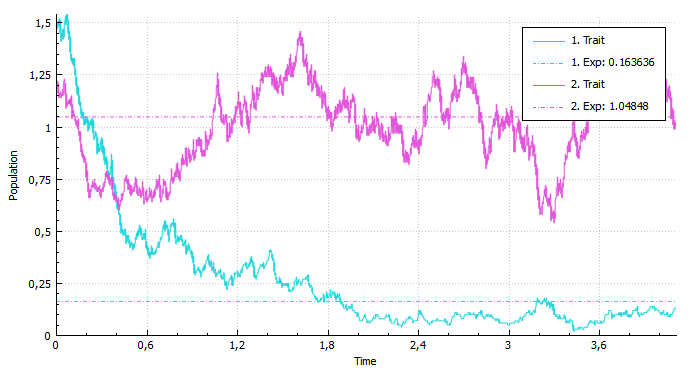
\includegraphics[width=0.7\linewidth]{./LPANormalisierungK100}
			\caption[LPAK100]{LPA Normalisierung mit K=100}
			\label{LPA Normalisierung K=100}
		\end{figure}
		\begin{figure}[H]
			\centering
			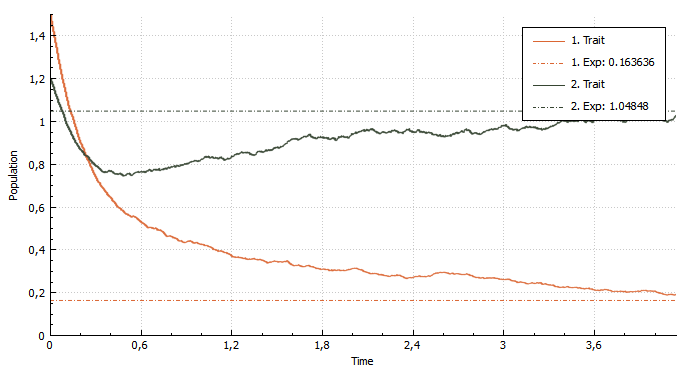
\includegraphics[width=0.7\linewidth]{./LPANormalisierungK10000}
			\caption[LPAK100]{LPA Normalisierung mit K=10000}
			\label{LPA Normalisierung K=10000}
		\end{figure}

		
		\subsubsection{Equilibrium}
		Man erkennt dass die Merkmale für $ K \to \infty $ eine Konvergenz gegen eine Funktion $ \xi_t = n_t \delta_x $ aufweist. Diese Funktion wiederum konvergiert gegen einen stabilen Zustand (im folgenden Equilibrium genannt), worin sich die Populationsgröße nicht mehr ändert. Diese sehen für monomorphe und dimorphe Populationen ohne Mutation folgendermaßen aus:
		\begin{itemize}
			\item Monomorphe Population\\
				\begin{align*}
				0 & = \dot{n} = (b(x) - d(x) - \bar{n}c(x,x))\bar{n}\\
				\bar{n} &= \frac{\left[ b(x)-d(x) \right]_+}{c(x,x)}
				\end{align*}
			\item Dimorphe Population\\
				\[ n_x = \frac{(b(x) - d(x))c(y,y)-(b(y)-d(y))c(x,y)}{c(y,y)c(x,x) - c(y,x)c(x,y)} \]
				\[ n = \frac{(b(y) - d(y))c(x,x)-(b(x)-d(x))c(y,x)}{c(y,y)c(x,x) - c(y,x)c(x,y)} \]
				oder $ (\bar{n}_x, 0)$, $ (0, \bar{n}_y)$ bzw. $ (0,0) $
		\end{itemize}
		Später im Kapitel TSS wird die Fitness Funktion eingeführt die näher erläutern kann wann welcher dimorphe stabile Zustand angenommen wird.
		In den Simulationen sind diese stabilen Zustände als gestrichelte Gerade angezeigt, gegen die Konvergenz stattfinden soll.
		
		
		
	\subsection{Algorithmus}
	Der Simulation liegt ein Algorithmus zugrunde der einen Sprung des Markov Sprung Prozesses durchführt. Im Code wird dazu die "{}EvolutionStep()"{} Funktion aufgerufen. (Es gibt auch Jump statt Step, aber mehrere Schritte)
	\begin{algorithm}[H]
		\caption{EvolutionStep()}
		\begin{algorithmic}[1]
			\ENSURE{A full evolution Step happened}
			\STATE calculateEventRates();
			\STATE sampleEventTime();
			\STATE changeATrait();
		\end{algorithmic}
	\end{algorithm}
	
	Von dieser werden folgende Berechnungen angestoßen:
		
	\begin{algorithm}[H]
		\caption{EvolutionStep()}
		\begin{algorithmic}[1]
			\ENSURE{A full evolution Step happened}
			\STATE ---$>$calculateEventRates();
			\STATE calculateTotalDeathRates()
			\STATE calculateTotalBirthRates()
			\STATE calculateTotalEventRate()
			\STATE ---$>$sampleEventTime();
			\STATE sampleEventTime();
			\STATE ---$>$changeATrait();
			\STATE choseTraitToChange();
			\STATE choseEventType();
			\STATE executeEventTypeOnTrait();
		\end{algorithmic}
	\end{algorithm}
	Schließlich der Ablauf der tatsächlichen Berechnung:
	\begin{algorithm}[H]
		\caption{EvolutionStep()}
		\begin{algorithmic}[1]
			\ENSURE{A full evolution Step happened}
			\REQUIRE $ t, X = \{0,\dots, n-1\} $
			\STATE ---$>$calculateEventRates();
			\FOR{ $ x \in X $ }
				\STATE $  D(x) := n_t(x) \cdot \left( d(x) + \sum_{y \in X} c(x,y) \cdot n_t(y) \right) $
				\STATE $ B(x) := \underbrace{b(x) \cdot (1 - \mu) \cdot n_t(x)}_{arteigene}  $
				\IF{$ x > 0 $}
					\STATE $ B(x) += \underbrace{b(x-1)\cdot n_t(x-1)}_{Mutation Links} \cdot \frac{\mu}{2} $
				\ENDIF
				\IF{$ x < n-1 $}
					\STATE $ B(x) += \underbrace{b(x+1)\cdot n_t(x+1)}_{Mutation Rechts} \cdot \frac{\mu}{2} $
				\ENDIF
				\STATE $ TotalTraitRate(x) = B(x) + D(x) $
			\ENDFOR
			\STATE $ TotalEventRate := \sum_{x \in X} TotalTraitRate(x) $
			
			\STATE ---$>$sampleEventTime();
			\STATE sample $ Z \sim exp(TotalEventRate) $
			\STATE $ t += Z $
			
			\STATE ---$>$choseTraitToChange();
			\STATE sample $ Y \sim U(0,TotalEventRate) $
			\FOR{$ x \in X $}
				\IF{$ Y \le TotalTraitRate(x) $}
					\STATE $ ChosenTrait := x $
					\STATE break
				\ENDIF
				\STATE $ Y -= TotalTraitRate(x) $
			\ENDFOR
			
			\STATE ---$>$choseEventType();
			\STATE sample $ Y \sim U(0,TotalTraitRate(ChosenTrait)) $
			\IF{$ Y \le B(ChosenTrait) $}
				\STATE isBirht := true
			\ELSE
				\STATE isBirth := false
			\ENDIF
			
			\STATE ---$>$executeEventTypeOnTrait();
			\IF{isBirth}
				\STATE $ n_t(ChosenTrait) += 1 $
			\ELSE
				\IF{$ n_t(ChosenTrait) \ge 0 $}
					\STATE $ n_t(ChosenTrait) -= 1 $
				\ENDIF
			\ENDIF
		\end{algorithmic}
	\end{algorithm}

	
	\subsection{Simulation}
	Nun kommen wir zur eigentlichen Simulation. Damit ist sowohl die Darstellung als auch die Programmarchitektur gemeint. 
		\subsubsection{Aufgabenteilung und Flexibilität}
		Die Idee der getrennten Aufgabenbereiche geht darauf zurück dass eine möglichst große Unabhängigkeit zwischen Arbeitsschritten notwendig ist um das Programm flexibel zu halten und sogenannten "{}Coderot"{} - "{}faulen Code"{} zu verhindern. Das bedeutet dass das Programm mit steigender Komplexität zunehmend unflexibler wird, also das Hinzufügen weiterer Features oder das Ändern/Verbessern zu sogenanntem "{}undefiniertem Verhalten"{} führt. (kurze Erklärung zum Begriff).\\
		Die Architektur des Programms kann grob in drei Module gefasst werden. 
		\begin{figure}[H]
			\centering
			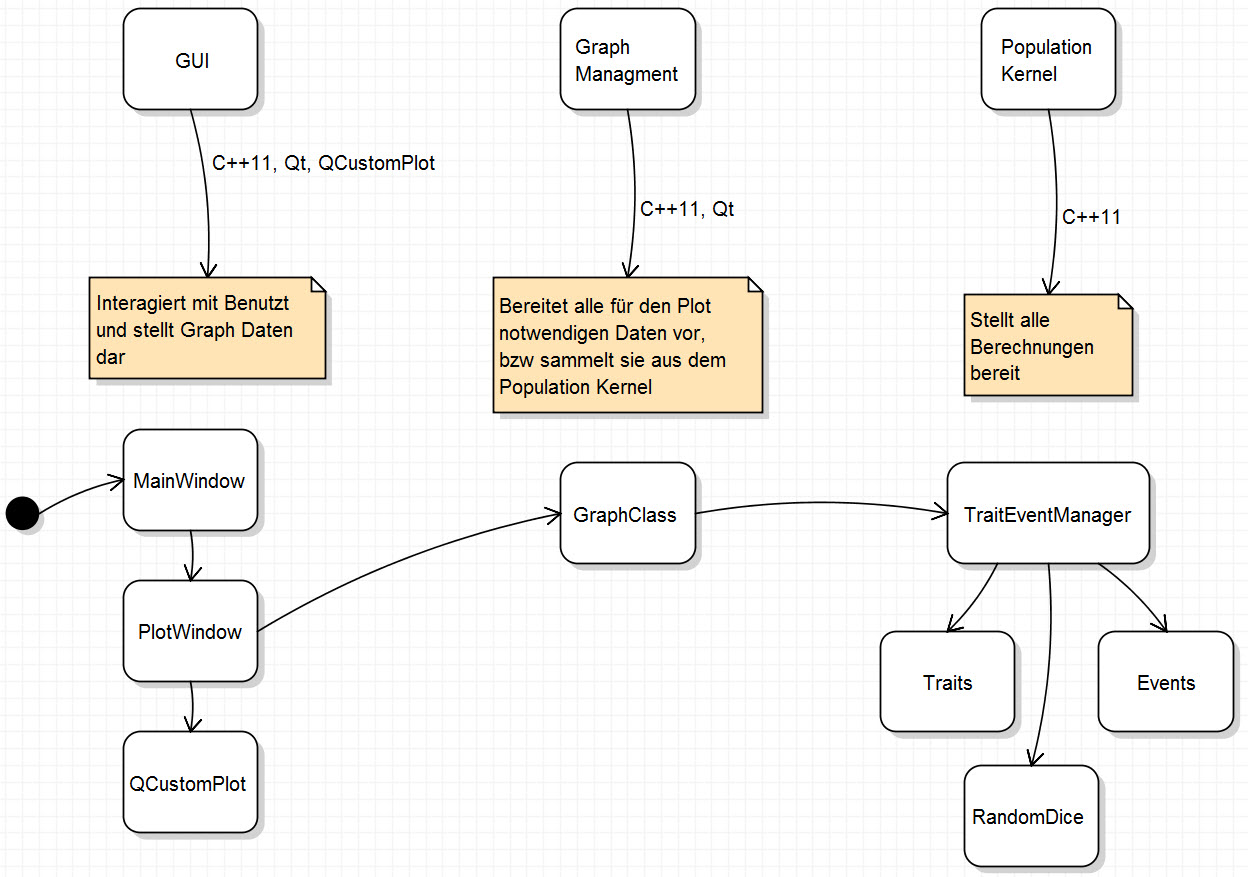
\includegraphics[width=0.7\linewidth]{./Bild_Module}
			\caption[Module]{Arbeitsmodule und Klassenabhängigkeiten}
			\label{Module und Klassen}
		\end{figure}
		Innerhalb der Arbeitsschritte sollte dabei genau die selbe Regel der Unabhängigkeit gelten wie bei den Modulen.
		
		\subsubsection{Layout}
		\begin{itemize}
			\item Die Bedienung des Programms sollte das lesen und Anzeigen der Merkmals-Parameter bereitstellen. Da es viele Parameter gibt und die Anzahl der Parameter quadratisch mit der Anzahl der betrachteten Merkmale steigt, bietet sich das Lesen aus zuvor beschriebenen Dateien an.
			\begin{figure}[H]
				\centering
				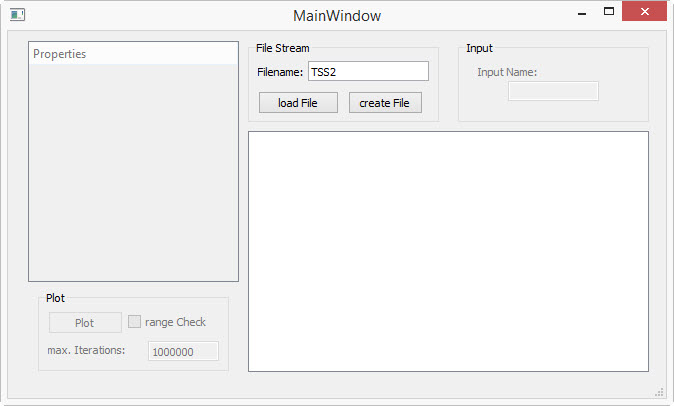
\includegraphics[width=0.7\linewidth]{./MainWindow_Start}
				\caption[Startwindow]{MainWindow nach dem Start}
				\label{MainWindow_Start}
			\end{figure}

			Zur Darstellung der gelesenen Parameter habe ich ein Baumstruktur gewählt.
			\begin{figure}[H]
				\centering
				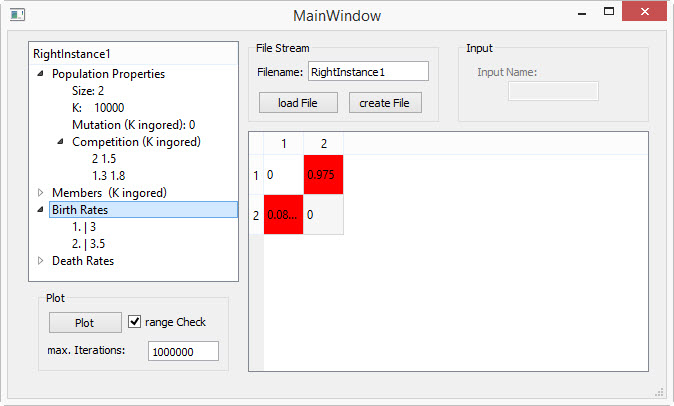
\includegraphics[width=0.7\linewidth]{./MainWindow_ParameterBaum}
				\caption[MainWindow_Parameter]{MainWindow mit geladenen Parametern}
				\label{Baumstruktur}
			\end{figure}
			\item Die letzte Herausforderung bestand darin eine Instanz durch das Programm geleitet erstellen zu können. Während diese Aufgabe bei einer Konsolenanwendung (bekannt aus den klassischen c Programmen) denkbar einfach mit "{}printf"{} und "{}scanf"{} erledigt werden konnte, sollte bei einem GUI eine Lösung her die Inputkonflikte verhindert und das Einlesen der Daten denkbar einfach macht. Dafür war es sinnvoll "{}Enter"{} als Bestätigung abzufangen und sicherzustellen dass der Curser nur innerhalb des gewünschten Feldes bleibt.
			\begin{figure}[H]
				\centering
				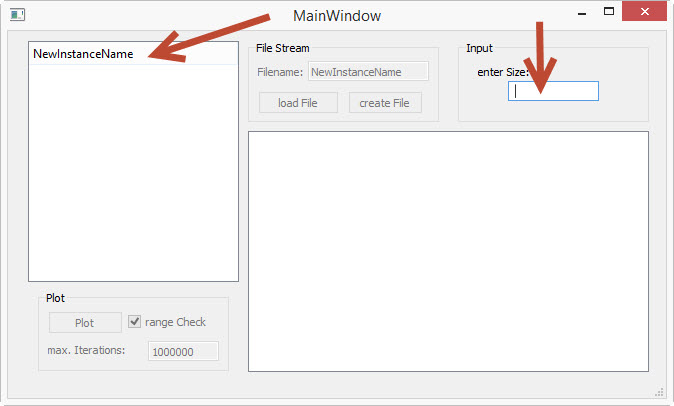
\includegraphics[width=0.7\linewidth]{./MainWindow_createFile}
				\caption[erstelle Datei]{Nach Klick auf "{}create File"{} werden die neuen Parameter einzeln abgefragt}
				\label{fig:MainWindow_createFile}
			\end{figure}
			\begin{figure}[H]
				\centering
				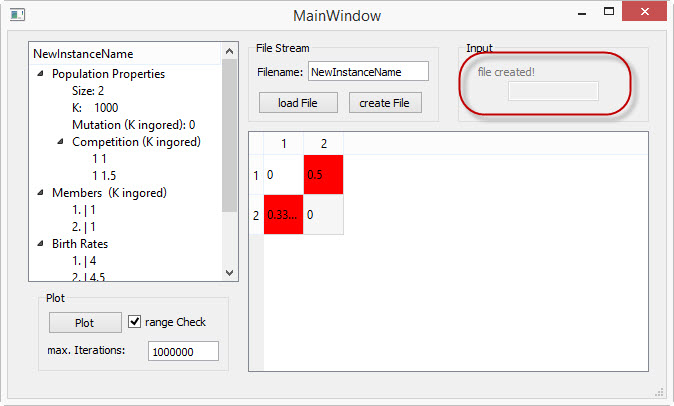
\includegraphics[width=0.7\linewidth]{./MainWindow_FileCreated}
				\caption[Datei erstellt]{Nach Eingabe des letzten Parameters}
				\label{fig:MainWindow_FileCreated}
			\end{figure}

		\end{itemize}
		Was die Darstellung der Graphen angeht, hat sich ein einfaches Bild des fertigen Plots durchgesetzt, wobei das Zoomen und ziehen des Bildes notwendige Elemente zur Untersuchung des Graphen sind. Zusätzlich ist es notwendig viele Bilder vergleichen zu können. Hierfür wurde das Abspeichern des Bildes gewünscht.\\
		Die Simulation wird gestartet nachdem man auf den "{}Plot"{} Button drückt. Dabei wird ein neues Fenster geöffnet.
		\begin{figure}[H]
			\centering
			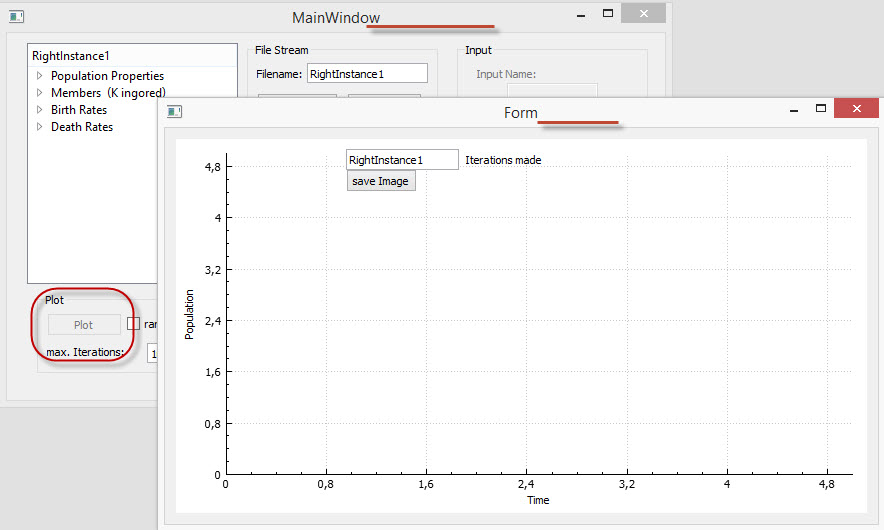
\includegraphics[width=0.7\linewidth]{./PlotWindow_start}
			\caption[PlotWindow_start]{Start des PlotWindow}
			\label{PlotWindow_start}
		\end{figure}
		Sobald der Plot Button gedrückt wurde und das Fenster angezeigt wird, arbeitet die Simulation bereits im Hintergrund in einem eigenen Thread. Dort werden alle notwendigen Iterationen bzw. Sprünge der Population durchgeführt ohne den Hauptthread damit zu belasten.\\ Während dieser Arbeiterthread aktiv arbeitet wird der "{}Plot"{} Button ausgegraut um mehrfaches Auslösen zu vermeiden und um anzuzeigen dass die Rechnung im Gange ist.\\
		Der Arbeiterthread gewährleistet nicht nur eine flüssige Interaktion mit dem Programm, sondern verhindert auch effektiv dass das Betriebssystem denkt das Programm wäre Abgestürzt oder würde nicht mehr ordnungsgemäß funktionieren. Das würde sonst folgendes evtl. bekannte Bild hervorrufen:
		\begin{figure}[H]
			\centering
			
\includegraphics[width=0.7\linewidth]{./KeineRueckmeldung}
			\caption[Keine Rueckmeldung]{Hauptthread wurde überlastet}
			\label{Keine Rueckmeldung}
		\end{figure}
		Wenn die Simulation  einen gewünschten Zustand erreicht hat, oder die maximale Anzahl an gewünschten Iterationen absolviert hat, werden anschließend maximal 10mio Punkte auf dem Koordinatensystem zu Graphen verbunden. Das kann so aussehen:
		\begin{figure}[H]
			\centering
			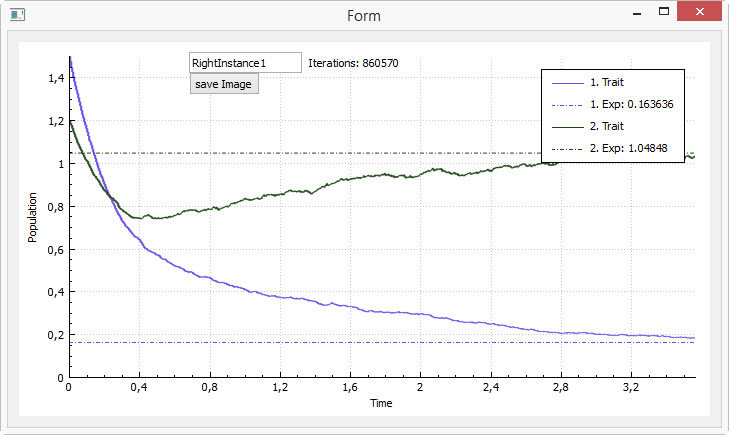
\includegraphics[width=0.7\linewidth]{./PlotWindow_smallBPDL}
			\caption[PlotWindow]{PlotWindow mit Dimorpher Population}
			\label{PlotWindow}
		\end{figure}
		
		
	\subsection{Korrektheit der Implementation}
	(Korrektheit des Algorithmus nicht notwendig bzw möglich)
	Ein ganz besonders interessantes Thema ist die Korrektheit der Implementation. Diese ist generell mit steigender Komplexität schwerer zu prüfen (besonders bei Zufallsbedingten Simulationen).\\
	Daher habe ich das Prinzip der "{}Testgetriebene Entwicklung"{}  (Test Driven Develeopment) verwendet.\\
	Dabei werden Funktionen des Programms unter vorher festgelegten Bedingungen laufen gelassen und mit einem erwarteten Verhalten verglichen. Das Ergebnis ist eine Ausgabe für Erfolg oder Misserfolg des Tests. Folgend ein Beispiel für eine Implementation eines einfachen Tests der prüft ob alle Parameter korrekt aus der Datei in die Objekte geschrieben werden.
	\begin{figure}[H]
		\centering
		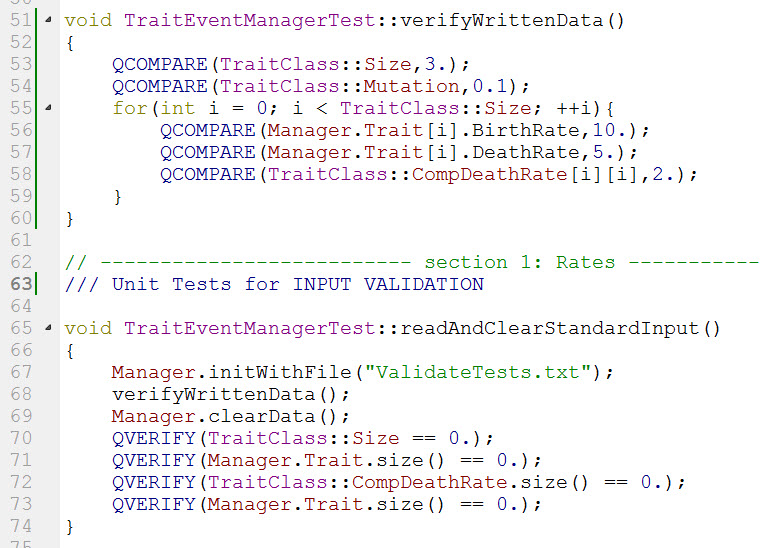
\includegraphics[width=0.7\linewidth]{./UnitTest}
		\caption[UnitTest]{UnitTest versichert korrektes lesen von Parametern aus Datei}
		\label{Unit Test}
	\end{figure}
	Anschließend ein Beispiel für einen Durchlauf der Testfunktionen:
	\begin{figure}[H]
		\centering
		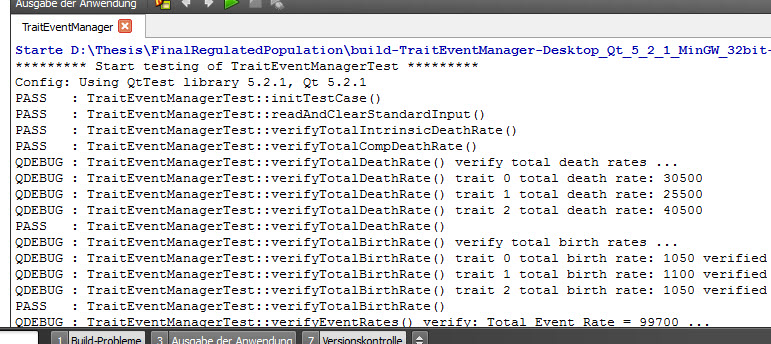
\includegraphics[width=0.7\linewidth]{./TestResult_start}
		\caption[Test Resultat einer Test Datei]{Ergebnisse einiger Tests}
		\label{Test Results}
	\end{figure}
	Die Testfunktionen zeigen auch dass eine komplexe Verwendung der Simulationen über die graphische Darstellung hinaus einfach realisierbar ist.
	
	\subsection{TSS}
	Bei TSS Prozessen beobachten wir wie sich Merkmale gegeneinander durchsetzten und sich verdrängen. (Tafelbild)\\
	Genau wie bei der LPA-Normalisierung ergeben sich TSS-Prozesse(Trait Substitution Sequence) als Grenzprozesse von BPDL-Prozessen. Zu der LPA-Normalisierung sollten jedoch mit größer werdendem K die Mutationen seltener werden ($ \frac{1}{e^{VK}} << \mu_K << \frac{1}{K log(K)} $) , also die Mutationswahrscheinlichkeit gegen 0 streben. Skaliert man nun noch zusätzlich die Zeit, so führt dies dazu, dass die Zeit, die ein Merkmal benötigt, um sich gegenüber einem anderen durchzusetzen und dieses zu verdrängen, infinitesimal klein wird. Somit simulieren die TSS-Prozesse eine Population, die zu jedem Zeitpunkt monomorph ist und sich im entsprechenden (für $ K < \infty $ angepassten) Equilibrium befindet.\\
	Spätestens jetzt wird die Fitness-Funktion interessant:
	\[ f(x,y) = b(x) - d(x) - c(x,y)\bar{n}_y \]
	Diese Fitness-Funktion gibt an, wie gut sich ein Merkmal gegenüber einem anderen durchsetzen kann. Sie ist die asymptotische Wachstumsrate von y, wenn x sich im Gleichgewichtszustand $ \bar{n}_x $ befindet und nur wenige Individuen von Typ y in der Population vorhanden sind. In der Simulation sieht man die Fitness der Merkmale zueinander in einer Matrix nach dem Laden der Parameter.
	\begin{figure}[H]
		\centering
		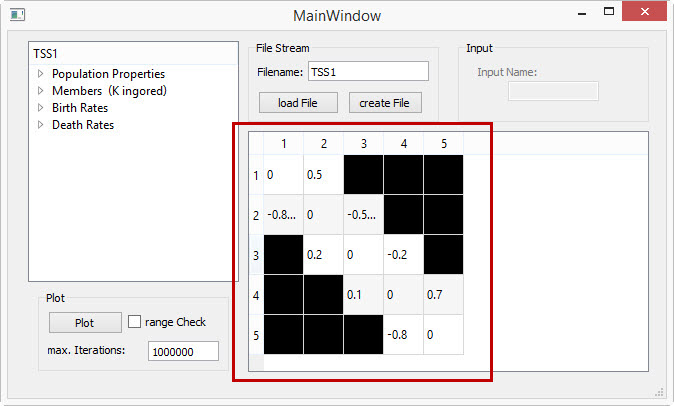
\includegraphics[width=0.7\linewidth]{./MainWindow_BandMatrix}
		\caption[Fitness Matrix]{Fitness Bandmatrix}
		\label{MainWindow mit Fitness Bandmatrix}
	\end{figure}
	Mit der Fitness kann man eine Konvergenz der Wahrscheinlichkeit für das überleben einer Mutation vorhersagen:
	\[ \frac{\left[ f(y,x)\right]_+ }{b(y)} \]
	Da diese Wahrscheinlichkeit gerne bereits beim einlesen der Parameter angezeigt werden will, habe ich vor sie als farblich ansteigenden Akzent den Elementen der Zelle hinzuzufügen. Bisher wird in der Matrix etwas grün oder rot markiert. Rot falls eine Koexistenz vorliegt und grün wenn die Wahrscheinlichkeit für Dominanz des Mutanten über 50\% liegt.
	\begin{figure}[H]
		\centering
		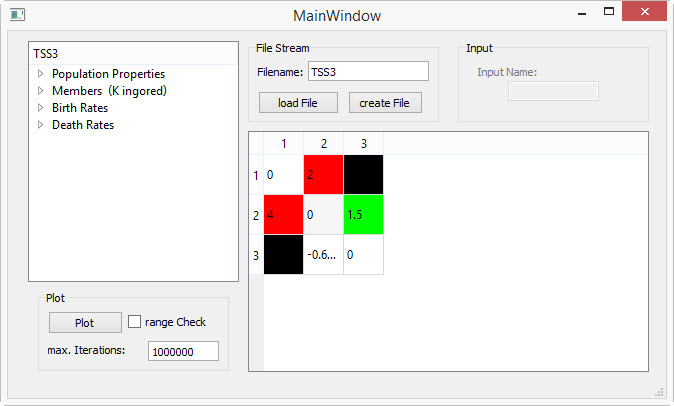
\includegraphics[width=0.7\linewidth]{./MainWindow_red_green_loaded}
		\caption[MainWindow_redGreenFitness]{Fitness Matrix mit roten und gruenen akzenten}
		\label{fig:MainWindow_red_green_loaded}
	\end{figure}
	Wenn der einfache BPDL Simulator für die Simulation dieses Prozesses verwendet werden würde, würde durch die seltenen Mutationen


	
	\subsection{Warum ist es vielleicht schwierig simple Mechanik einzupflegen?}
	Wie man sich vielleicht denken kann sind viele kleine Features an und für sich sehr simpel.
	Unglücklicherweise gibt es viele kleine solche Features und Daten die mit dem Programm verbunden wären. 

\newpage
\section{Achtes Treffen}
\subsection{Was ist geplant?}
\subsection{Was habe ich gemacht?}
\subsection{Bekannte Bugs}


\section{Weitere geplante Punkte}
\subsection{Offene Fragen}
	\begin{itemize}
		\item Soll die Mutationswahrscheinlichkeit für BPDL proportional zu K gestaucht werden oder auch wie bei TSS?
	\end{itemize}
\subsection{Bekannte Bugs}
	\begin{itemize}
		\item Fehler beim Laden nicht falsch eingetippter Instanznamen abfangen.
		\item Zeitlinie bei BPDL Programm. Wenn K 100 mal kleiner wird, so wird Die Zeit auch 100 mal kürzer. Sollte aber nicht passieren.
		\item Manchmal nicht korrektes Aussterben. Todespunkt wird nicht gemalt $ \Rightarrow $ wird als aktiv angezeigt.
	\end{itemize}
	
\subsection{große Verbesserungen}
	\begin{itemize}
		\item skalieren der interpolierten TSS stellen.
		\item Es wäre sinnvoll wenn es eine Möglichkeit gibt die angestrebten stabilen Zustände als Option auszuwählen welche angezeigt werden sollten. Dabei sollte die Beschriftung "{}Dimorph"{} oder "{}Monomporph"{} darin auftauchen.
		\item dynamisches Abbruchkriterium welches für alle TSS Instanzen angemessen terminiert.
		\item Dokumentation zu Programmcode und Bedienung
		\item Anpassen der neuen Geburten und Equilibrien.
		\item Evtl. Abfrage beim Überschreiben von Dateien
		\item Instanzexplorer
		\item GraphClass aufräumen (RangeCheck etc.)
		\item Unit Tests anpassen und mit TSS erweitern (und Mutation rate testen)
		\item Beim speichern die Zeit hinzufügen um das häufige überschreiben zu vermeiden.
		\item Release Version des Programms erstellen.
		\item Es wurde gewünscht dass irgendwo die Anzahl der Mutationen bis ein Switch von dominanten Merkmalen stattgefunden hat angezeigt wird.
		\item komplexere dimorphe stabile Zustände implementieren. Mit Rücksicht auf Fitness.
		\item dynamisches Zeichnen des Graphen mit "{}addData"{} und "{}replot"{}
	\end{itemize}

\subsection{kleine Verbesserungen}
	\begin{itemize}
		\item Sofortiges Laden der Instanz nach erstellen der neuen Testinstanz
		\item Was passierte wenn während eines Jumps eine Mutation stattfindet?
		\item Fitness Matrix beschriften
		\item Fenster benennen
		\item Items in der Tabelle sollten zentrieren
		\item Es sollte das aktuell verwendete K in der Simulation angezeigt werden.
		\item stabiler Zustand weniger Aufdringlich (z.B. größerer Abstand zwischen Strichen und geringere Strichstärke)
		\item Feedback beim Speichern eines Bildes
		\item Wenn Plot Button grau ist, soll der Buttontext deutlich machen dass simuliert (gearbeitet) wird. Vielleicht sogar mit "{}estimated time"{}.
		\item Überschrift bzw Namen der Fenster ändern.
	\end{itemize}



\end{document}
